\let\negmedspace\undefined
\let\negthickspace\undefined
\documentclass[journal,12pt,onecolumn]{IEEEtran}
\usepackage{cite}
\usepackage{amsmath,amssymb,amsfonts,amsthm}
\usepackage{algorithmic}
\usepackage{graphicx}
\graphicspath{{./figs/}}
\usepackage{textcomp}
\usepackage{xcolor}
\usepackage{txfonts}
\usepackage{listings}
\usepackage{enumitem}
\usepackage{mathtools}
\usepackage{gensymb}
\usepackage{comment}
\usepackage{caption}
\usepackage[breaklinks=true]{hyperref}
\usepackage{tkz-euclide} 
\usepackage{listings}
\usepackage{gvv}                                        
%\def\inputGnumericTable{}                                 
\usepackage[latin1]{inputenc}     
\usepackage{xparse}
\usepackage{color}                                            
\usepackage{array}                                            
\usepackage{longtable}                                       
\usepackage{calc}                                             
\usepackage{multirow}
\usepackage{multicol}
\usepackage{hhline}                                           
\usepackage{ifthen}                                           
\usepackage{lscape}
\usepackage{tabularx}
\usepackage{array}
\usepackage{float}
%\newtheorem{theorem}{Theorem}[section]
%\newtheorem{theorem}{Theorem}[section]
%\newtheorem{problem}{Problem}
%\newtheorem{proposition}{Proposition}[section]
%\newtheorem{lemma}{Lemma}[section]
%\newtheorem{corollary}[theorem]{Corollary}
%\newtheorem{example}{Example}[section]
%\newtheorem{definition}[problem]{Definition}

\begin{document}

\title{7.4.27}
\author{EE25BTECH11020 - Darsh Pankaj Gajare}
% \maketitle
% \newpage
% \bigskip
%\begin{document}
{\let\newpage\relax\maketitle}
%\renewcommand{\thefigure}{\theenumi}
%\renewcommand{\thetable}{\theenumi}
Question:\\
The triangle $PQR$ is inscribed in the circle $x^2+y^2=25$.If $\vec{Q}$ and $\vec{R}$ have co-ordinates $\brak{3,4}$ and $\brak{-4,3}$ respectively then $\angle QPR$ is equal to
\begin{multicols}{4}
	\begin{enumerate}
		\item $\frac{\pi}{2}$
		\item $\frac{\pi}{3}$
		\item $\frac{\pi}{4}$
		\item $\frac{\pi}{6}$
	\end{enumerate}
\end{multicols}
\solution
\begin{table}[H]
	\centering
	\caption{}
	\begin{tabular}{|c|c|}
\hline
\textbf{Name} & \textbf{Value} \\ \hline
$\vec{A}$ & $\myvec{2 & 1 \\0 & 3}$ \\ \hline
\end{tabular}

	\label{}
\end{table}
\begin{align}
\vec{x}^\top\vec{x} &= 25
\end{align}

The given points (position vectors) are
\begin{align}
\vec{q} &= \myvec{3\\4}, & \vec{r} &= \myvec{-4\\3}
\end{align}

Verify they lie on the circle:
\begin{align}
\vec{q}^\top\vec{q} &= 3^2+4^2 = 25, \\
\vec{r}^\top\vec{r} &= (-4)^2+3^2 = 25.
\end{align}

Compute the inner product (matrix/dot product):
\begin{align}
\vec{q}^\top\vec{r} &= \myvec{3 & 4}\myvec{-4\\3} \\
&= 3\cdot(-4) + 4\cdot 3 = -12 + 12 = 0.
\end{align}

Compute norms (using matrix notation) and the central angle $\theta$:
\begin{align}
\norm{\vec{q}} &= \sqrt{\vec{q}^\top\vec{q}} = 5, & 
\norm{\vec{r}} &= \sqrt{\vec{r}^\top\vec{r}} = 5, \\
\cos\theta &= \dfrac{\vec{q}^\top\vec{r}}{\norm{\vec{q}}\norm{\vec{r}}}
= \dfrac{0}{5\cdot 5} = 0 \\
\implies \theta &= \frac{\pi}{2}.
\end{align}

Since $\angle QPR$ is the angle subtended at the circumference by chord $QR$, it equals half the central angle:
\begin{align}
\angle QPR &= \frac{\theta}{2} = \frac{\pi}{4}.
\end{align}


Plot using C libraries:
\begin{figure}[H]
	\centering
	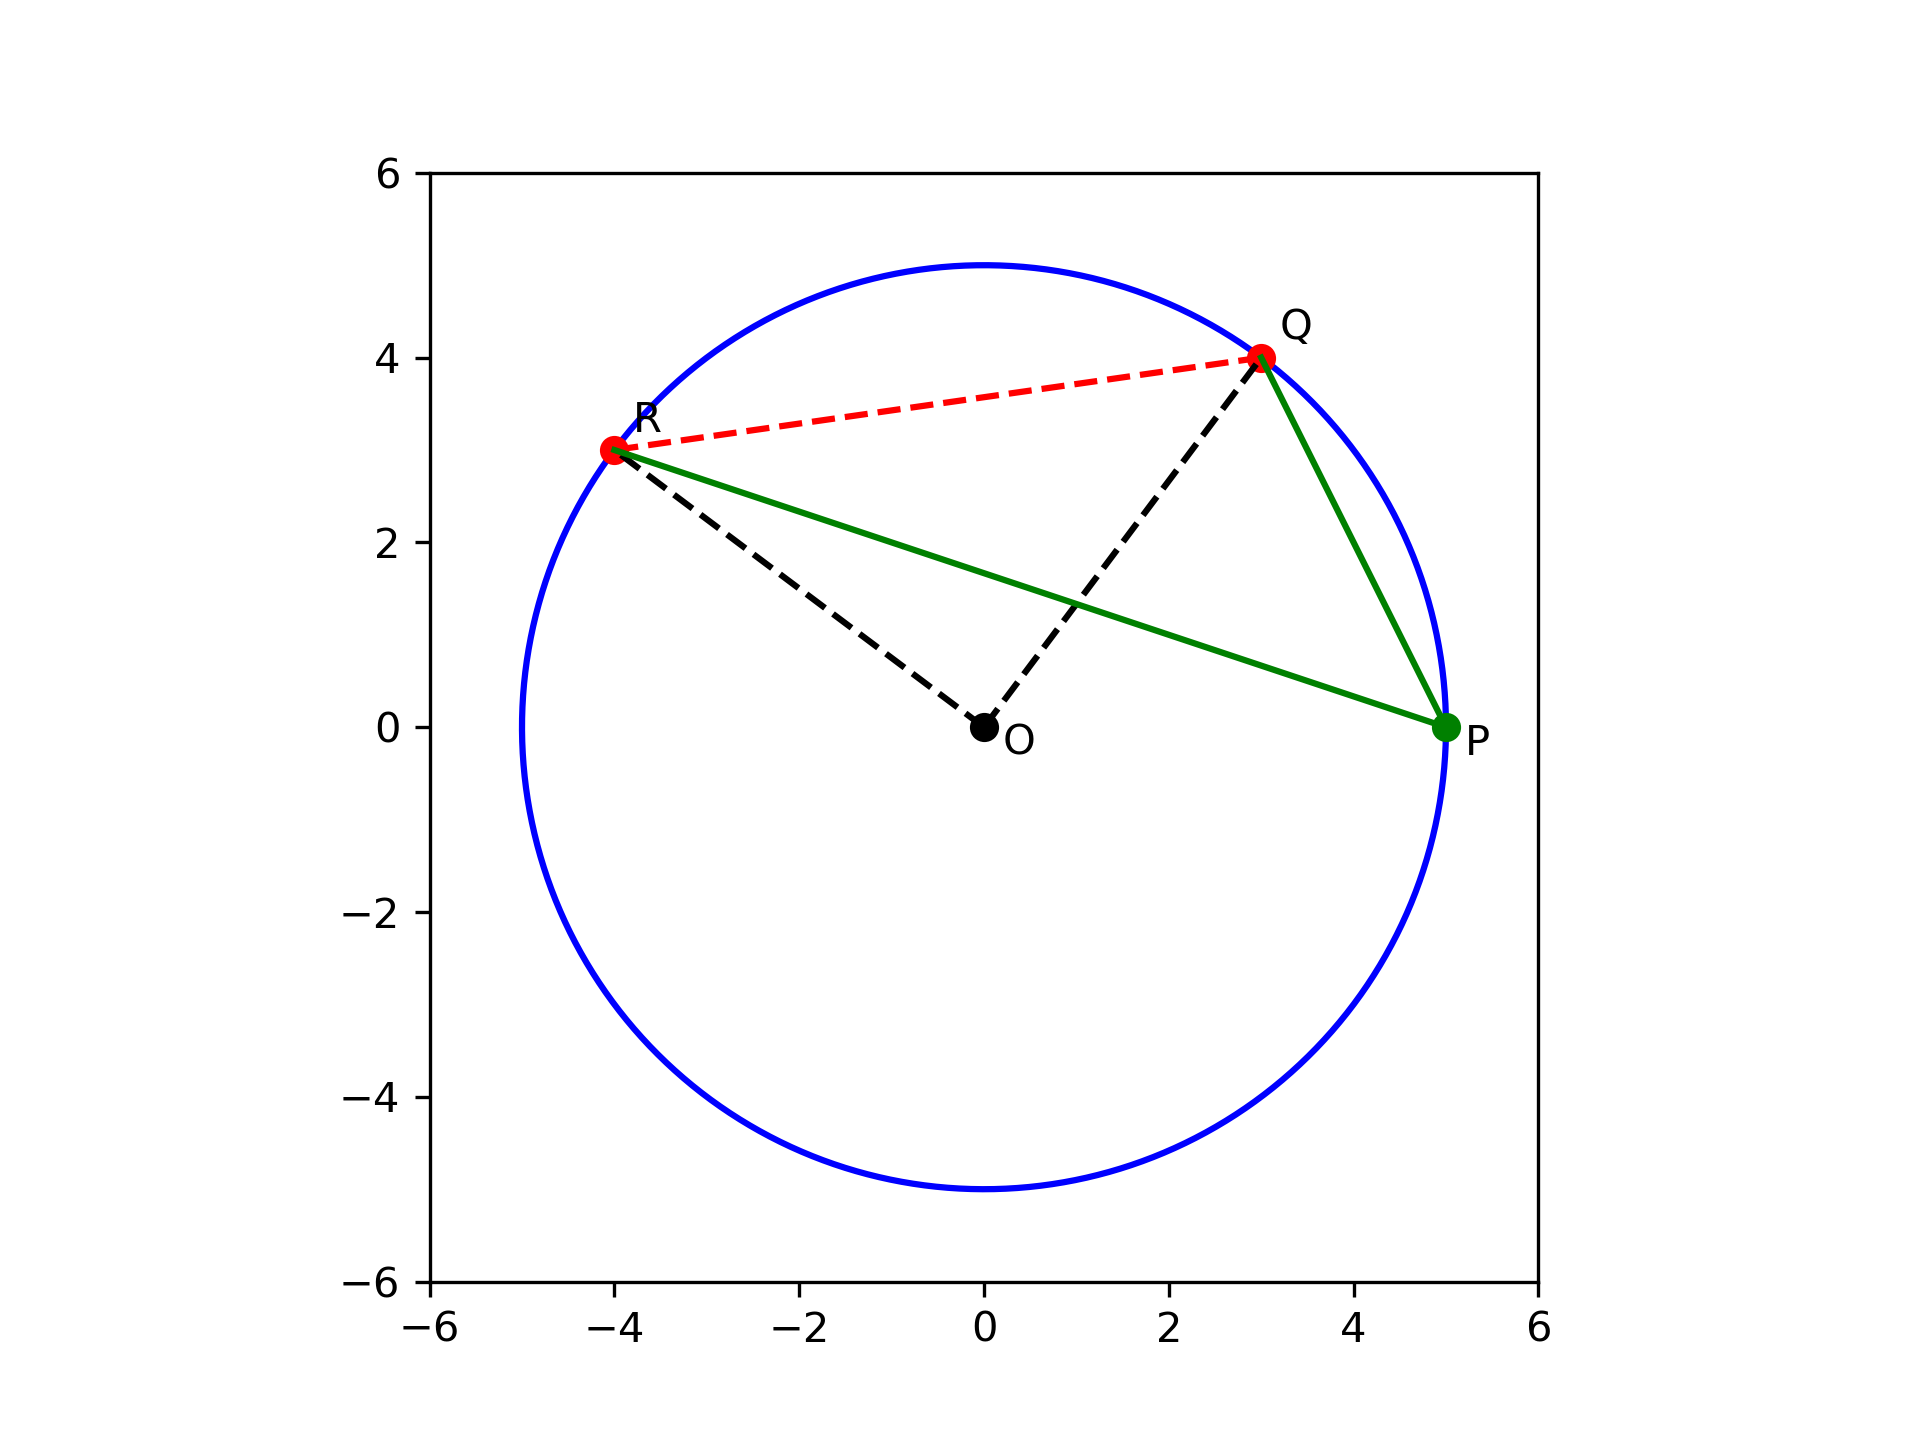
\includegraphics[scale=0.5]{img1}
	\caption*{}
	\label{img1}
\end{figure}
Plot using Python:
\begin{figure}[H]
	\centering
	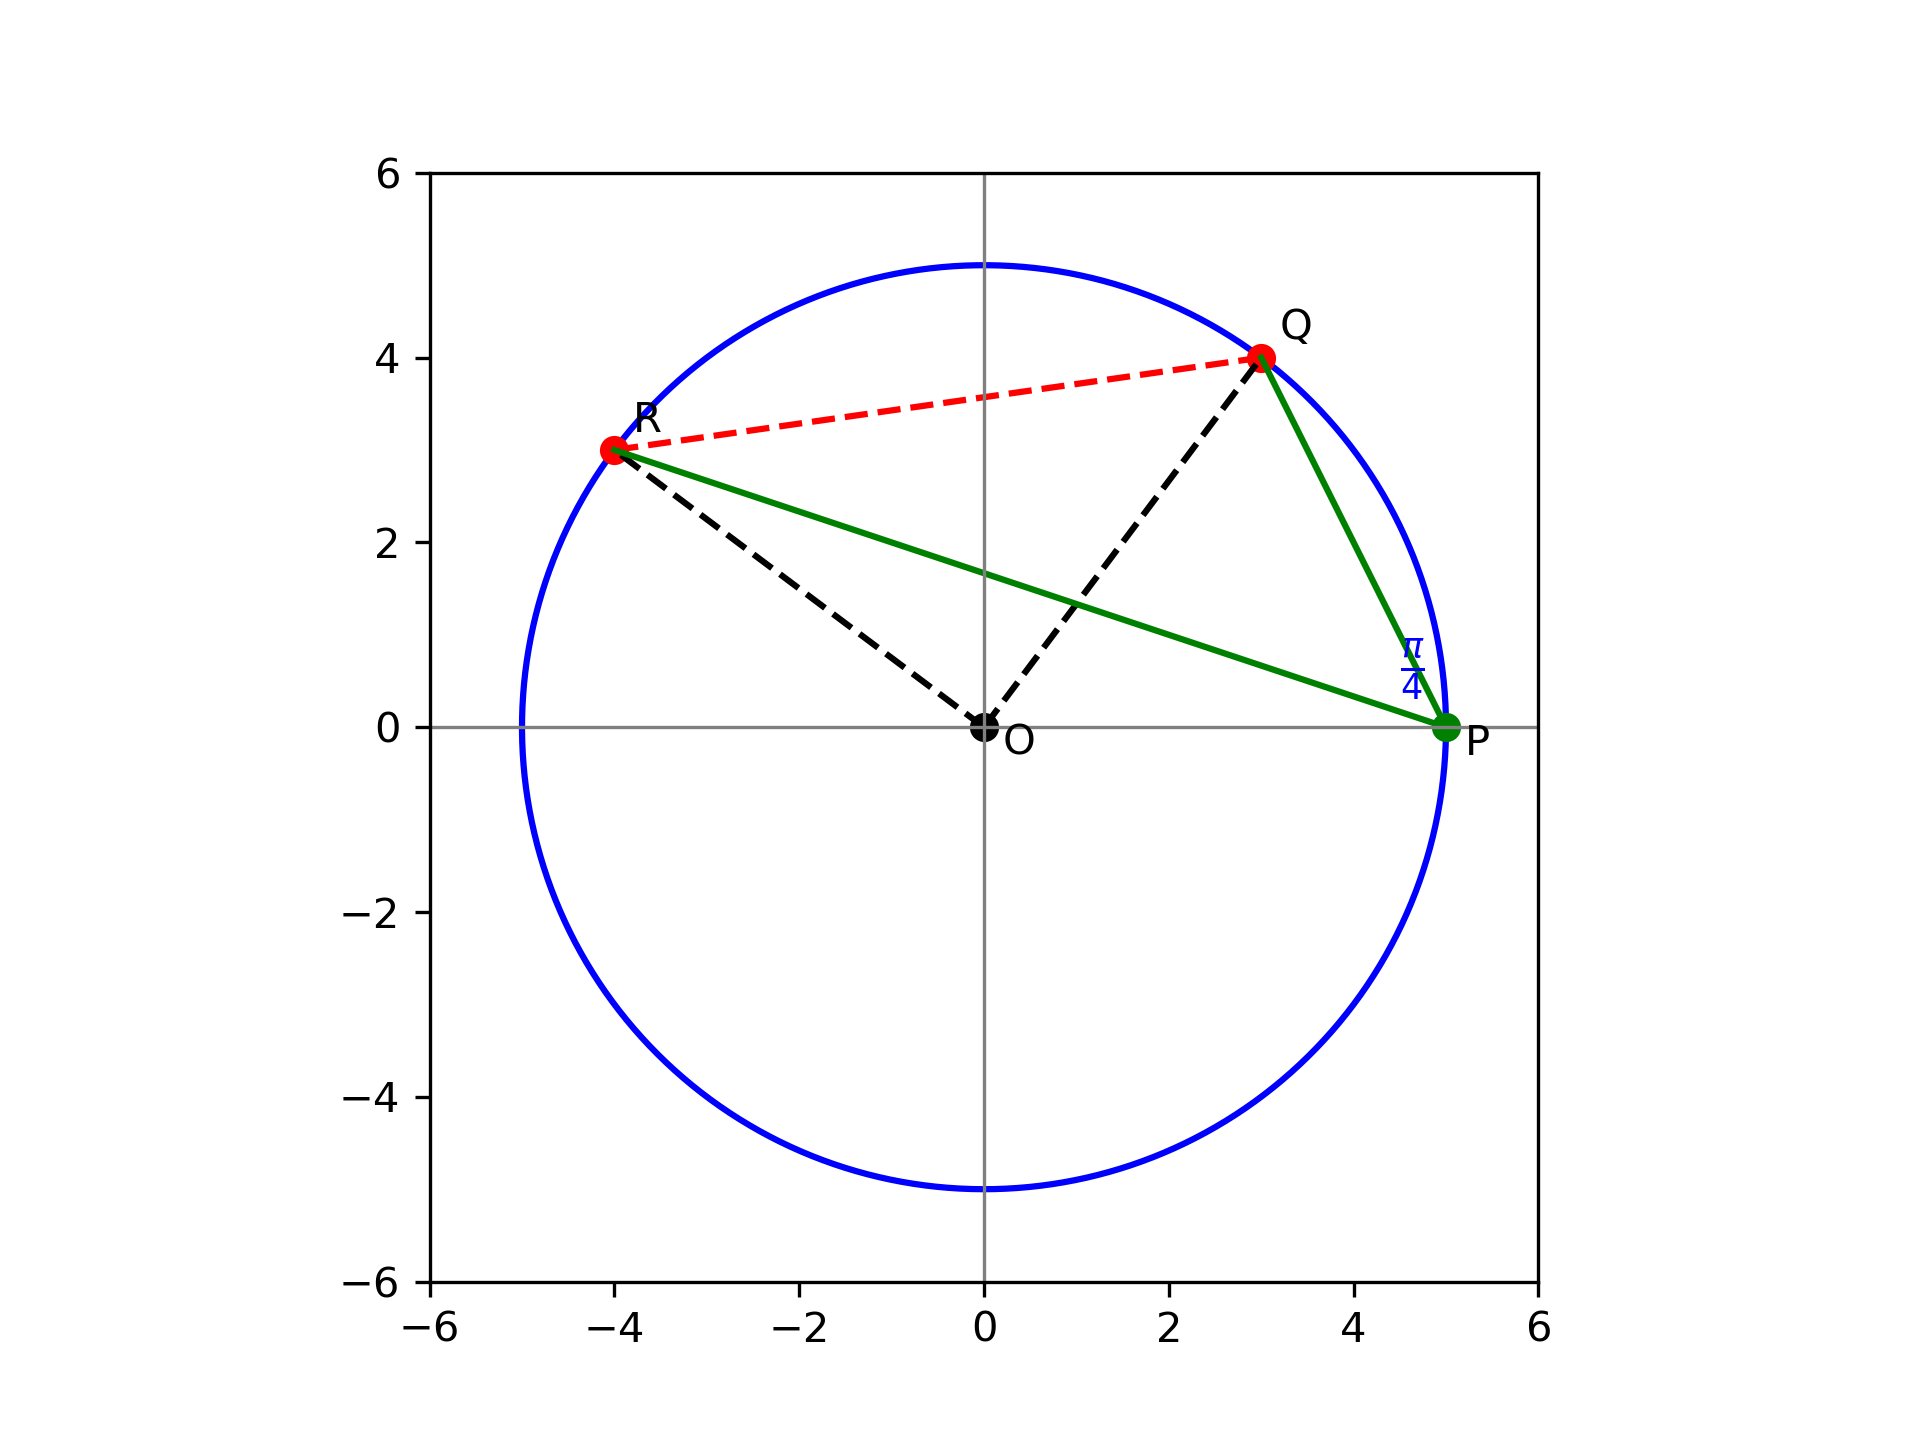
\includegraphics[scale=0.5]{img2}
	\caption*{}
	\label{img2}
\end{figure}
\end{document}

